\renewcommand{\theequation}{\theenumi}
\renewcommand{\thefigure}{\theenumi}
\renewcommand{\thetable}{\theenumi}
\begin{enumerate}[label=\thesection.\arabic*.,ref=\thesection.\theenumi]
\numberwithin{equation}{enumi}
\numberwithin{figure}{enumi}
\numberwithin{table}{enumi}

\item If calls arrive at a telephone exchange such that the time of arrival of any call is independent of the time of arrival of earlier or future calls, the probability distribution function of the toatl number of calls in a fixed time interval will be

\begin{enumerate}
\begin{multicols}{2}
\setlength\itemsep{2em}

\item Poisson
\item Gaussian
\item Exponential
\item Gamma

\end{multicols}
\end{enumerate}
\solution



\begin{table}[h!]
\centering
    \begin{tabular}{|p{0.14\linewidth}|p{0.35\linewidth}|p{0.16\linewidth}|p{0.16\linewidth}|}
    \hline
    \textbf{Symbol} & \textbf{Description} & \textbf{Property} & \textbf{Random}\\[0.5ex]
    \hline
    $T$ & Total time period & $T=n\Delta t$ &No\\
    \hline
    $n$ & Total Number of intervals &  &No\\
    \hline
    $\Delta t$ & One time interval & $\Delta t$=T/n & No\\
    \hline
    $k$ & Number of calls arrived during the time interval (0,$T$) & & Yes\\
    \hline
    $t_i$ & Denotes the time of arrival of each call in interval $(0,T)$ & &Yes\\
    \hline
    $p$ & Probability of receiving a call at time $t_i$ & &No\\
    \hline
    $\lambda$ & Average number of calls $(0,T)$ & $\lambda=np$ &No\\
    \hline
    $e$ & Euler's number & &No\\
    \hline
    \end{tabular}
\end{table}
Lets denote the fixed time interval by [0,$T$].
To find the probability of $k$ number of calls during this time interval, lets divide the interval into $n$ parts of equal length $\Delta t$.
Let us denote the probability of receiving a call at a particular time $t_i$ by $p$. Suppose the telephone exchange receives an average of $\lambda$ calls in time interval of length $T$.\\
Hence, we have
\begin{align}
    np=\lambda\\
    \implies p=\frac{\lambda}{n}
\end{align}
\begin{figure}[ht]
    \centering
    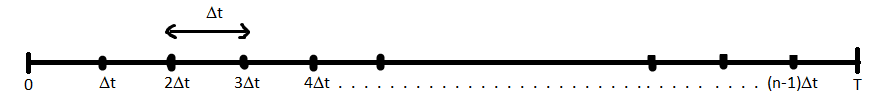
\includegraphics[width=\columnwidth]{solutions/ec/43/Figures/figure1.png}
    \caption{Figure showing division of time intervals}
    \label{ec43:figure_1}
\end{figure}
In Fig. \ref{ec43:figure_1}, the interval (0,$T$) has been divided into n equal parts, where length of each interval is $\Delta t$ and the number of calls in each interval is a random variable.
\begin{figure}[ht]
    \centering
    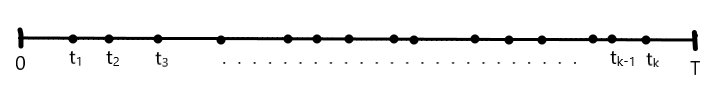
\includegraphics[width=\columnwidth]{solutions/ec/43/Figures/figure2.png}
    \caption{Figure showing times of arrival of $k$ calls}
    \label{ec43:Figure_2}
\end{figure}
$t_i$ where $i=\{1,2,3\cdots k\}$ are the time of arrival of $k$ calls in the interval $(0,T)$.\\

A call has probability $p$ for arriving at $t_i, \forall  i=\{1,2,\cdots k\}$ and the probability of 1-$p$ for not arriving at that instant.\\

In Binomial distribution we have certain number of intervals, i.e. $n$, with probability of arrival of each call as $p$ and for a binomial random variable $X=\{0,1\cdots n\}$, the probability of call arriving in any $k$ intervals is 
\begin{align}
    \pr{X=k}=\comb{n}{k}\cdot p^k\cdot(1-p)^k
\end{align} But in Poisson distribution, we essentially have infinite intervals, so $n\rightarrow\infty$. Thus, the probability expression changes to:
\begin{align}
   \lim_{n \to \infty}\pr{X=k}=\lim_{n \to \infty}\frac{n!}{k!(n-k)!}\left(\frac{\lambda}{n}\right)^k\left(1-\frac{\lambda}{n}\right)^{n-k}
\end{align}
\begin{multline}  \label{ec43:5}
    \lim_{n \to \infty}\pr{X=k}=\\
    \left(\frac{\lambda^k}{k!}\right)\lim_{n \to \infty}\frac{n!}{(n-k)!}\left(\frac{1}{n}\right)^k\left(1-\frac{\lambda}{n}\right)^n\left(1-\frac{\lambda}{n}\right)^{-k}
\end{multline}
Now lets take the limit of right-hand side one term at a time. We’ll do this in three steps. The first step is to find the limit of 
\begin{equation}
\begin{split}\label{ec43:6}
     \lim_{n \to \infty}\frac{n!}{(n-k)!n^k}
     &= \lim_{n \to \infty}\frac{n(n-1)(n-2)..(n-k+1)}{n^k}\\
    & = \lim_{n \to\infty}\left(\frac{n}{n}\right)\left(\frac{n-1}{n}\right)....\left(\frac{n-k+1}{n}\right)\\
   &= \lim_{n \to \infty}\left(1-\frac{1}{n}\right)\left(1-\frac{2}{n}\right)...\left(1-\frac{k-1}{n}\right)\\
    &=1\cdot1\cdot1........1\\
    &=1   
    \end{split}
\end{equation}
Now we have to find the limit of 
\begin{align}\label{ec43:7}
    \lim_{n \to \infty}\left(1-\frac{\lambda}{n}\right)^n 
\end{align}
We know that the definition $e$ is given as 
\begin{align}
    e=\lim_{x \to \infty}\left(1+\frac{1}{x}\right)^x
\end{align}
So, lets replace the value of $-\frac{n}{\lambda}$ by x in \eqref{ec43:7}, we get
\begin{align}\label{ec43:9}
    \lim_{n \to \infty}\left(1-\frac{\lambda}{n}\right)^n =\lim_{x \to \infty}\left(1+\frac{1}{x}\right)^{x(-\lambda)}=e^{-\lambda}
\end{align}
And the third part is to find the limit of 
\begin{align}
    \lim_{n \to \infty}\left(1-\frac{\lambda}{n}\right)^{-k}
\end{align}
As n approaches infinity, this term becomes $1^{-k}$ which is equal to one.
So,
\begin{align}\label{ec43:11}
    \lim_{n \to \infty}\left(1-\frac{\lambda}{n}\right)^{-k}=1
\end{align}
Now on substituting \eqref{ec43:6}, \eqref{ec43:9} and \eqref{ec43:11} in equation \eqref{ec43:5}, we get
\begin{multline}  
    \left(\frac{\lambda^k}{k!}\right)\lim_{n \to \infty}\frac{n!}{(n-k)!}\left(\frac{1}{n}\right)^k\left(1-\frac{\lambda}{n}\right)^n\left(1-\frac{\lambda}{n}\right)^{-k}=\\
    \left(\frac{\lambda^k}{k!}\right)(1)\left(e^{-\lambda}\right)(1)
\end{multline}
This just simplifies into
\begin{align}\label{ec43:final_equation}
    \pr{X=k}=\left(\frac{\lambda^k e^{-\lambda}}{k!}\right)
\end{align}
   \eqref{ec43:final_equation} is equal to probability density function of Poisson distribution, which gives us probability of $k$ successes per period, with given parameter of $\lambda$.\\
   
   $\therefore $The probability distribution function of the total
number of calls in a fixed time interval will be \textbf{Poisson} distribution.\\
Answer: Option(A)



%
\item Let $X$ be the Poisson random variable with parameter $\lambda$ = 1. Then, the probability 
$\pr{2 \leq X \leq 4}$ equals ............
%
\\
\solution

Let 
\begin{align}
	X\in \{0,1,2,3,4,5...\}
\end{align}
We know that, for a poisson random variable $X$ with a given parameter $\lambda$, probability of $X=k$ is:
\begin{align} \label{eq_0}
	\pr{X=k}=\left(\frac{\lambda^k e^{-\lambda}}{k!}\right)	
\end{align}
CDF is:
\begin{align}
    F(X=k)=\sum_{x=0}^{k}\left(\frac{\lambda^x e^{-\lambda}}{x!}\right)
\end{align}
   
% The graph of CDF is shown below
% \includegraphics[width=\linewidth]{cdf.png}
And also,
\begin{align}
    \Pr\brak{x < X \le y} = F\brak{y} - F\brak{x}\label{eq_1}
\end{align}
Now by using \eqref{eq_1},
\begin{align}
    \pr{2 \leq X \leq 4} 
    & = \pr{1 < X \leq 4}\\
    & = F(4)-F(1)\\
    & = \frac{65}{24e}-\frac{2}{e}\\
    & = \frac{17}{24e}
\end{align}
\begin{figure}[ht]
    \centering
    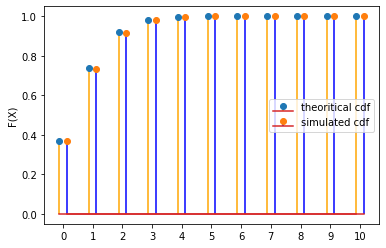
\includegraphics[width=\columnwidth]{solutions/xe/2019/simulated_theoritical.png}
    \caption{Theoretical CDF vs Simulated CDF}
    \label{Figure_0}
\end{figure}

%
\item  Suppose $p$ is the number of cars per minute passing through a certain road junction between $5$ $PM$ and $6$ $PM,$ and $p$ has a Poisson distribution with mean $3$. What is the probability of observing fewer than $3$ cars during any given minute in this interval$?$
\begin{enumerate}
    \item $8/(2e^3)$
    \item $9/(2e^3)$
    \item $17/(2e^3)$
    \item $26/(2e^3)$
\end{enumerate}
\solution

Probability of Poison Distribution is,
\begin{align}
    \pr{X=p}=\frac{e^{-\mu}\mu^p}{p!}
\end{align}
Here, $p$ refers to no. of cars per minute,
$p \in \{0,1,2,\dots,\infty\}$
Mean of poison distribution,
\begin{align}
    \mu=3
\end{align}
\begin{align}
    \pr{X=p}=\frac{e^{-3}3^p}{p!}
\end{align}
\begin{table}[h!]
\centering
\caption{Table of probability of no. of cars passing per minute}
\resizebox{\columnwidth}{!}{
  \begin{tabular}{||c|c|c|c|c|c||}
    \hline
    $p$ & $0$ & $1$ & $2$ & $3$ & \dots\\
    \hline
    \hline
    $\pr{X=p}$ & $1/e^3$ & $3/e^3$ & $9/(2e^3)$ & $9/(2e^3)$ & \dots\\
    \hline
  \end{tabular}
  \label{Table1}
}
\end{table}
by Boolean logic,
\begin{align}
    \pr{X<3}=\pr{X=0}+\pr{X=1}+\pr{X=2}
\end{align}
\begin{align}
    \pr{X<3}=\frac{17}{2e^3}
\end{align}
Option $(C)$ is correct

%
\item Let $X$ be the Poisson random variable with parameter $\lambda$ = 1. Then, the probability 
$\pr{2 \leq X \leq 4}$ equals ............
%
\solution

Let 
\begin{align}
	X\in \{0,1,2,3,4,5...\}
\end{align}
We know that, for a poisson random variable $X$ with a given parameter $\lambda$, probability of $X=k$ is:
\begin{align} \label{eq_0}
	\pr{X=k}=\left(\frac{\lambda^k e^{-\lambda}}{k!}\right)	
\end{align}
CDF is:
\begin{align}
    F(X=k)=\sum_{x=0}^{k}\left(\frac{\lambda^x e^{-\lambda}}{x!}\right)
\end{align}
   
% The graph of CDF is shown below
% \includegraphics[width=\linewidth]{cdf.png}
And also,
\begin{align}
    \Pr\brak{x < X \le y} = F\brak{y} - F\brak{x}\label{eq_1}
\end{align}
Now by using \eqref{eq_1},
\begin{align}
    \pr{2 \leq X \leq 4} 
    & = \pr{1 < X \leq 4}\\
    & = F(4)-F(1)\\
    & = \frac{65}{24e}-\frac{2}{e}\\
    & = \frac{17}{24e}
\end{align}
\begin{figure}[ht]
    \centering
    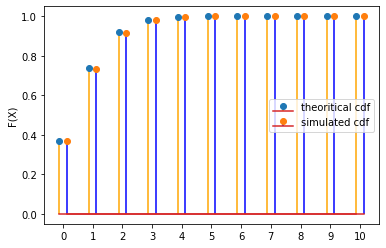
\includegraphics[width=\columnwidth]{solutions/xe/2019/simulated_theoritical.png}
    \caption{Theoretical CDF vs Simulated CDF}
    \label{Figure_0}
\end{figure}

%
\item Customers arrive at a shop according to Poisson distribution with a mean of 10 customers/hour. The manager notes that no customer arrives for the first 3 minutes after the shop opens. The probability that a customer arrives within the next 3 minutes is

%
\solution
Given, 
mean of 10 customers arrive in a time interval of 60 minutes $\iff$ mean of $\dfrac{t}{6}$ customers arrive in a time interval of t minutes,
Customers arrive according to Poisson distribution with a mean of $\dfrac{t}{6}$ customers/t minutes,
\begin{align}
\therefore \lambda = \frac{t}{6} \label{me/2021/33/a}
\end{align}
Let $X$ denotes the number of customers in first t minutes,$Y$ denotes the number of customers in second t minutes.
according to  poisson distribution,
\begin{align}
\pr{X=x}= e^{-\lambda} \frac{\lambda^{x}}{x\,!} \label{me/2021/33/b}
\end{align}
using \eqref{me/2021/33/a} in \eqref{me/2021/33/b},
\begin{align}
\pr{X=x}= e^{-\frac{t}{6}} \frac{(\frac{t}{6})^{x}}{x\,!} \label{me/2021/33/c}
\end{align}
 the probability that a customer arrives within the next t minutes given that no customer arrives for the first t minutes after the shop opens,which can also be written as,
\begin{align}
\pr{Y\neq 0|X=0}=\frac{\pr{Y\neq 0,X=0}}{\pr{X=0}}
\end{align}
\begin{table}[ht]
\caption{Probability distribution for values of X and Y}
\begin{center}
    \begin{tabular}{|c|c|c|}
    \hline
     & P(X)&P(Y)\\
    \hline
    0& $e^{-\frac{t}{6}}$& $e^{-\frac{t}{6}}$\\
    \hline
    1 & $\frac{t e^{-\frac{t}{6}}}{6}$ & $\frac{t e^{-\frac{t}{6}}}{6}$\\
    \hline
    \end{tabular}
\end{center} 
\end{table}
As the arrival of customers in second t minutes does not depend on the arrival of customers in first t minutes, X and Y are independent,
\begin{align}
\pr{Y\neq 0|X=0}&=\frac{\pr{Y\neq 0}\pr{X=0}}{\pr{X=0}}\\
&=\pr{Y\neq 0}\\
&= 1-\pr{Y=0} 
\end{align}
using \eqref{me/2021/33/c},
\begin{align}
\pr{Y\neq 0|X=0}&=1- e^{-\frac{t}{6}}
\end{align}
we need to find the probability for t=3,the required probability is given by,
\begin{align}
&=1- e^{-\frac{1}{2}}\\
&=0.3935
\end{align}

%
\item  Consider a single machine workstation to which jobs arrive according to a
Poisson distribution with a mean arrival rate of 12 jobs/hour. The process
time of the workstation is exponentially distributed with a mean of 4
minutes. The expected number of jobs at the workstation at any given
point of time is \ldots (\textit{round off to the nearest integer}).
%
\solution
In a Poisson process,
 \begin{align}
          \pr{X=x}&= e^{-\lambda \Delta t} \frac{(\lambda \Delta t)^{x}}{x\,!}
 \end{align}
If $\Delta t \rightarrow 0$ then probability of having only one Poisson job is  
  \begin{align}
         \pr{X=1}=\lambda \Delta t \label{me2021-42:singlejob-condition}
 \end{align}
 Some assumptions:\\
 In time interval $\Delta t$,
 \begin{itemize}
     \item Exactly one job is arrived  
     \item or Exactly one job is completed
     \item or Nothing happens
 \end{itemize}
Assumptions seem quite reasonable as $\Delta t$ is very small then the probability of occurrence of more than one poisson job is very low.\\
 For job arrival,
 \begin{itemize}
 \item It is distributed according to Poisson distribution.
     \item Its
 Rate parameter $\lambda $=12 jobs/hour.
 \item Using \eqref{me2021-42:singlejob-condition},Probability that a single job arrives in a small interval $\Delta t=\lambda\Delta t$.
 \end{itemize}
 For Job completions,
 \begin{itemize}
     \item  Job completion time is distributed exponentially with mean of 4 minutes 
     \item Then we can assume that no. of job completions are distributed as Poisson distribution with rate parameter $\mu$ = 15 jobs/hour
     \item Once again using \eqref{me2021-42:singlejob-condition},
 Probability that a single job will be completed in a small interval $\Delta t=\mu \Delta t$
 \end{itemize}
 Some notations,
 \begin{table}[h]
\begin{tabular}{|c|p{6cm}|}
\hline
\textbf{Parameter} & \textbf{Definition}                               \\ \hline
$\lambda$          & Poisson rate parameter for the arrival of jobs    \\ \hline
$\mu$              & Poisson rate parameter for the completion of jobs \\ \hline
$\lambda \Delta t$ & Probability that a single job arrives in a small interval $\Delta t$\\\hline 
$\mu \Delta t$ & Probability that a single job will be completed in a small interval $\Delta t$\\\hline 
$P_j(t)$             & probability of having j jobs at workstation at time t \\\hline
$\pi_j$            & steady probability of having j jobs at workstation\\\hline
\end{tabular}
\caption{Parameters and their definitions used in the problem}
\label{me2021-42:tab:parameters}
\end{table}
 \begin{itemize}
     \item  Initial no.of jobs at workstation is 0.
     \item Let $P_{j}(t)$ denote the probability of having $j$ jobs waiting at the workstation at the time $t$ for this initial case.
     \item After a long time,probability of having  j jobs becomes steady.
     \item Let us denote steady state probability of having j jobs as $\pi_j$.
 \end{itemize}
 Condition which ensures that steady state is reached is
 \begin{align}
     \diff{P_j(t)}{t}&=0\\
     \lim_{\Delta t\rightarrow 0}\dfrac{P_j(t+\Delta t)-P_j (t)}{\Delta t}&=0\label{me2021-42:steady-condition}
 \end{align}
  We can reach a state of $j$ jobs at time $t+\Delta t$ from
  \begin{itemize}
      \item A state of $j-1$ jobs at time $t$ with a new job arriving in the next $\Delta t$
      \item A state of $j+1$ jobs at time $t$ with a job completing in the next $\Delta t$
      \item A state of $j$ jobs at time $t$ and nothing happening in the next $\Delta t$
  \end{itemize}
 Assuming time  $t$ is long enough for the occurrence of steady state.The above relations can be shown in probability equations as:  
 \begin{align}
     P_j(t+\Delta t)&=P_{j-1}(t)\lambda\Delta t+ P_{j+1}(t)\mu \Delta t \nonumber\\&+P_j (t) (1-\lambda\Delta t -\mu \Delta t)\\
     \dfrac{P_j(t+\Delta t)-P_j (t)}{\Delta t}&= P_{j-1}(t)\lambda +P_{j+1}(t)\mu\nonumber\\& - P_j(t)\lambda -P_j(t)\mu
\end{align}
Using \eqref{me2021-42:steady-condition} we get,
\begin{align}
     \implies P_{j-1}(t)\lambda +P_{j+1}(t)\mu&=P_j(t)\lambda +P_j(t)\mu \\
     \pi_{j-1}\lambda +\pi_{j+1}\mu&=\pi_j\lambda +\pi_j\mu\label{me2021-42:recursive} 
 \end{align}
 Note that the above equations are  for $j \geq 1$. \\
 For j=0 jobs at time $t+\Delta t$ we can reach it from j=1 job at time $t$ with a job completion in the next $\Delta t$ or else stay at j=0 at time $t$ and do nothing the next $\Delta t$
\begin{align}
    P_0(t+\Delta t)&=P_1(t)\mu \Delta t+\nonumber\\&~~~~P_0(t)(1-\lambda \Delta t)\\
    \dfrac{P_0(t+\Delta t)-P_0(t)}{\Delta t}&=P_1(t) \mu \Delta t-P_0(t)\lambda \Delta t
\end{align}
Once again using \eqref{me2021-42:steady-condition},we will get,
\begin{align}
    P_0(t)\lambda \Delta t&= P_1(t) \mu \Delta t\\
    P_0(t)\lambda&=P_1(t) \mu \\
    \pi_0 \lambda&=\pi_1\mu\label{me2021-42:base}
\end{align}
Solving \eqref{me2021-42:base} and \eqref{me2021-42:recursive} with appropriate j one by one,we will get $P_j$ in terms of $P_0$ as
\begin{equation}
    P_j=\brak{\dfrac{\lambda}{\mu}}^jP_0 
\end{equation}
consider $\rho = \dfrac{\lambda}{\mu}$.
\begin{table}[h]
\begin{tabular}{|c|p{6cm}|}
\hline
\textbf{Parameter} & \textbf{Definition}                               \\ \hline
$E(j)$             & Expected no. of jobs at workstation \\ \hline
$\rho$             & $\dfrac{\lambda}{\mu}$\\\hline
\end{tabular}
\caption{Parameters and their definitions used in the problem}
\label{me2021-42:tab:parameters}
\end{table}
\begin{equation}
    P_j=\rho^j P_0 \label{me2021-42:solution}
\end{equation}
We can prove that \eqref{me2021-42:solution} is indeed the solution of recursion equation \eqref{me2021-42:recursive} by using mathematical induction.\\
Assuming $\rho<1$,let us calculate $P_0$ in terms of $\rho$
\begin{align}
    \sum_{j=0}^{\infty}P_j&=1\\
    \sum_{j=0}^{\infty}\rho^j P_0 &=1\\
    \dfrac{P_0}{1-\rho}&=1\\
    P_0&=1-\rho
\end{align}
This yields,\\
\begin{equation}
    P_j=\rho^j(1-\rho)
\end{equation}
Let us calculate expected value of jobs waiting at workstation.
\begin{align}
    E(j)&=\sum_{j=0}^{\infty}jP_j\\
    E(j)&=(1-\rho)\sum_{j=0}^{\infty}j\rho^j\label{me2021-42:first}\\
    \rho E(j)&=(1-\rho)\sum_{j=0}^{\infty}j\rho^{j+1}\\
    \rho E(j)&=(1-\rho)\sum_{j=1}^{\infty}(j-1)\rho^{j}\label{me2021-42:second}
\end{align}
Subtracting \eqref{me2021-42:second} from \eqref{me2021-42:first}.we get,
\begin{align}
    (1-\rho)E(j)&=(1-\rho)\sum_{j=1}^{\infty}\rho^j\\
    E(j)&=\sum_{j=1}^{\infty}\rho^j\\
    E(j)&=\dfrac{\rho}{1-\rho}\label{me2021-42:expect}
\end{align}
In our case $\rho=\dfrac{\lambda}{\mu}=\dfrac{12}{15}=\dfrac{4}{5}$.\\\\Substituting it in the \eqref{me2021-42:expect} we get,\\
\begin{equation}
    E(j)=4
\end{equation}
$\therefore$ Expected no.of jobs at workstation is 4.


%
\item Cars arrive at a service station according to Poisson's distribution with a mean rate of 5 per hour.The service time per car is exponential with a mean of 10 minutes.At a steady state,the average waiting time in the queue is 
%
\solution
This problem can be solved using Queuing theory.But first we have to understand queuing theory.
\begin{itemize}
\item In queuing theory we try to determine what happens when people join in queue.
\item\textbf{Parameters for measuring Queuing performance}
\begin{enumerate}
    \item $\lambda$ = Average arrival time
    \item $\mu$ = Average service time
    \item $\rho$ = Utilization factor
    \item $L_q$ = Average number in the queue
    \item $L$ = Average number in the system
    \item $W_q$ = Average waiting time
    \item $W$ = Average time in the system
    \item $P_n$ = Steady state probability of exactly n customers in the system
\end{enumerate}
\item Typically most of the times arrivals follow poisson distribution and services follow exponential distributions.
\item The given question only has one queue so we can conclude that it is a single server model and there is no limit for number of cars in the queue so we can say that it is "\textbf{M/M/1:/$\infty$/$\infty$/FIFO}" by kendall's notation (or) usually "\textbf{M/M/1}" 
\item Here '\textbf{M}' indicates the memory less property of the model first \textbf{M} is for arrival and second one for service and 1 is the number of servers in the model and '$\infty$' indicates the limit of the queue and second '$\infty$' represent population and '\textbf{FIFO}' represents First-In First-Out service.
\item \textbf{NOTE:} In cases where there is no limit in the queue we only take the cases where $\frac{\lambda}{\mu}<1$. Otherwise there could be customers who will not get their service. \newline The memory less property allows us to assume that one event can take place in a small interval of time. The event could be either a arrival or a service.
\item\textbf{Deriving formulas :}
 For the time interval($t,t+h$), where $h \to 0$
\begin{align}
    \Pr{(\text{1 arrival})}&=\lambda h\\
    \Pr{(\text{1 service})}&=\mu h\\
    \Pr{(\text{no arrival})}&=1-\lambda h\\
    \Pr{(\text{no service})}&=1-\mu h
\end{align}
\begin{multline}
    P_{n}(t+h)=P_{n-1}(t)\times\Pr{(\text{1 arrival})}\times\Pr{(\text{no service})}\\
    +P_{n+1}(t)\times\Pr{(\text{no arrival})}\times\Pr{(\text{1 service})}\\
    +P_n(t)\times\Pr{(\text{no arrival})}\times\Pr{(\text{no service})}\label{me2011-19:eq:eq1}
\end{multline}
\begin{multline}
    \implies P_{n}(t+h)=P_{n-1}(t)(\lambda h)(1-\mu h)\\
    +P_{n+1}(t)(\mu h)(1- \lambda h)\\
    +P_n(t)(1-\lambda h)(1-\mu h)
\end{multline}
Now, Neglecting higher order terms of $h$.
\begin{multline}
    \implies P_{n}(t+h)=P_{n-1}\lambda h+P_{n+1}\mu h\\
    +P_n(t)(1-\lambda h-\mu h)
\end{multline}
\begin{multline}
    \implies \frac{P_n(t+h)-P_n(t)}{h}=P_{n-1}(t)\lambda+P_{n+1}(t)\mu\\
    -P_n(t)(\lambda+\mu)
\end{multline}
At steady state, $P_n(t+h)=P_n(t)$
\begin{align}
    \implies\lambda P_{n-1}+\mu P_{n+1}&=(\lambda+\mu)P_n\label{me2011-19:eq:res1}
\end{align}
Now, calculating $P_0(t+h)$ using \eqref{me2011-19:eq:eq1}
\begin{multline}
    P_0(t+h)=P_1(t)(1-\lambda h)(\mu h)\\
    +P_0(t)(1-\lambda h)
\end{multline}
Again, Neglecting higher order terms of $h$
\begin{multline}
    \implies P_0(t+h)=P_1(t)(\mu h)\\
    +P_0(t)(1-\lambda h)
\end{multline}
\begin{align}
    \implies\frac{P_0(t+h)-P_0(t)}{h}&=P_1(\mu)-P_0(\lambda)
\end{align}
At steady state, $P_0(t+h)=P_0(t)$
\begin{align}
    \implies \mu P_1&=\lambda P_0\label{me2011-19:eq:eq2}\\
    \implies P_1&=\brak{\frac{\lambda}{\mu}}P_0\label{me2011-19:eq:res2}
\end{align}
Using \eqref{me2011-19:eq:res1} by substituting $n=1$
\begin{align}
    \lambda P_0+\mu P_2&=(\lambda+\mu)P_1\\
    \implies \lambda P_0+\mu P_2&=\lambda P_1+\mu P_1
\end{align}
from \eqref{me2011-19:eq:eq2} and \eqref{me2011-19:eq:res2}
\begin{align}
    \implies\lambda P_0+\mu P_2&=\lambda P_1+\lambda P_0\\
    \implies P_2&=\brak{\frac{\lambda}{\mu}}P_1\\
    \implies P_2&=\brak{\frac{\lambda}{\mu}}^2P_0\label{me2011-19:eq:eq3}
\end{align}
We assume $\frac{\lambda}{\mu}=\rho$ and generalize $P_n$ by \eqref{me2011-19:eq:res2} and \eqref{me2011-19:eq:eq3}
\begin{align}
  P_n&=\brak{\frac{\lambda}{\mu}}^nP_0\\
  \implies P_n&=\rho^nP_0\label{me2011-19:eq:res3}
\end{align}
We know that sum of all probabilities equal to 1
\begin{align}
    \sum_{i=1}^{\infty}P_i&=1\\
    \implies P_0+P_1+P_2+....&=1
\end{align}
Using \eqref{me2011-19:eq:res3}
\begin{align}
    \implies P_0+\rho P_0+\rho^2P_0+....&=1\\
    \implies P_0\brak{1+\rho+\rho^2+...}&=1\\
    \implies P_0\brak{\frac{1}{1-\rho}}&=1\\
    \implies P_0&=1-\rho\label{me2011-19:eq:res4}\\
    \therefore P_n=\rho^n(1-\rho)
\end{align}
The number of people in the system ($L_s$) is the expected value
\begin{align}
    L_s&=\sum_{i=0}^{\infty}iP_i\\
    \implies L_s&=\sum_{i=0}^{\infty}i\rho^iP_0\\
    \implies L_s&=\rho P_0\sum_{i=0}^{\infty}i\rho^{i-1}\\
    \implies L_s&=\rho P_0\sum_{i=0}^{\infty}\frac{d}{d\rho}\brak{\rho^i}\\
    \implies L_s&=\rho P_0\frac{d}{d\rho}\sum_{i=0}^{\infty}\rho^i\\
    \implies L_s&=\rho P_0\frac{d}{d\rho}\brak{\frac{1}{1-\rho}}\\
    \implies L_s&=\rho P_0\frac{1}{(1-\rho)^2}
\end{align}
By using \eqref{me2011-19:eq:res4}
\begin{align}
    \implies L_s&=\rho(1-\rho)\frac{1}{(1-\rho)^2}\\
    \implies L_s&=\frac{\rho}{1-\rho}
\end{align}
We can also say that the number of people beign served is $\rho$
\begin{align}
    \therefore L_s&=L_q+\text{people beign served}\\
    \implies L_s&=L_q+\rho\\
    \implies L_q&=L_s-\rho\\
    \implies L_q&=\frac{\rho}{1-\rho}-\rho\\
    \implies L_q&=\frac{\rho^2}{1-\rho}
\end{align}
\newpage
The relation between $L_s$ and $W_s$ and $L_q$ and $W_q$ are the Little's equation and they are related as
\begin{align}
    L_s&=\lambda W_s\\
    L_q&=\lambda W_q
\end{align}
\end{itemize}
\section{Solution}
From the question given,
\begin{align}
    \lambda &=5\text{hr}^{-1}\\
    \mu&=\frac{1}{10}\text{min}^{-1} =6\text{hr}^{-1}
    \end{align}
Therefore,
\begin{align}
    \text{Utilization rate}(\rho)&=\frac{\lambda}{\mu}=\frac{5}{6}
    \end{align}
Average number (or) length in queue be $L_q$
    \begin{align}
    L_q&=\frac{\rho^2}{1-\rho}\\
    &=\frac{\brak{\frac{5}{6}}^2}{1-\frac{5}{6}}\\
    &=\frac{25}{6}
    \end{align}
Let the Average waiting time in queue be $W_q$
    \begin{align}
    W_q&=\frac{L_q}{\lambda}\\
    &=\frac{\frac{25}{6}}{5}\\
    &=\frac{5}{6}\text{hr}=50\text{min}
\end{align}
The average waiting time in the queue is 50 min.
\newpage
\begin{table}[h!]
\centering
\resizebox{\columnwidth}{!}
{
    \begin{tabular}{|c|c|}
    \hline
    Parameter & Value \\
    \hline
    $\lambda$ & $5$hr$^{-1}$\\
    \hline
    $\mu$ & $6$hr$^{-1}$\\
    \hline
    $\text{Utilization rate}\brak{\rho}=\frac{\lambda}{\mu}$ & $\frac{5}{6}$\\[1ex]
    \hline
    $\text{Length in queue}\brak{L_q}=\frac{\rho^2}{1-\rho}$ & $\frac{25}{6}$\\[1ex]
    \hline
    $\text{Waiting time in queue}\brak{W_q}=\frac{L_q}{\lambda}$ & $\frac{5}{6}$hr\\[1ex]
    \hline     
    \end{tabular}
}
    \caption{Parameters of the given question and values.}
    \label{me2011-19:TABLE-1}
\end{table}
%
\item The number $N$ of persons getting injured in a bomb blast at a busy market place is a random variable having a Poisson Distribution with parameter $\lambda(\geq 1)$.
 A person injured in the explosion may either suffer a minor injury requiring first aid or suffer a major injury requiring hospitalisation. Let the number of persons with minor injury be $N_1$ and the conditional distribution of $N_1$ given N is
 \begin{align}
     \pr{N_1 = i \vert N} = \frac{1}{N}
     \label{condition}
 \end{align}
 Find the expected number of persons requiring hospitalisation.
 %
\solution
We know,
\begin{align}
    \pr{A|B} = \frac{\pr{A\cap B}}{\pr{B}}
\end{align}
Also, for a Poisson Distribution:
\begin{align}
    \pr{N = x} = \frac{e^{-\lambda}\lambda^x}{x!}
    \label{poisson}
\end{align}
where $\lambda$ is the parameter\\
Let $N_2$ be the number of persons hospitalised.\\
Let $N = a$, and $N_1 = i(i\leq a)$, then, $N_2 = a-i$\\
Then, from \eqref{condition} and \eqref{poisson}:
\begin{align}
    \pr{N_2 = a-i} =\pr{N_1 = i}\\
    =\pr{N_1 = i|N = a}\pr{N = a}\\
     = \frac{1}{a}\frac{e^{-\lambda}\lambda^a}{a!}
\end{align}
Thus,
\begin{align}
    E(N_2) = \sum_{a = 0}^{\infty} \sum_{i = 0 }^{a} (a-i) \times \frac{1}{a}\frac{e^{-\lambda}\lambda^a}{a!}\\
     = \sum_{a=0}^{\infty}\frac{e^{-\lambda}\lambda^a}{a!} \sum_{i = 0 }^{a} \frac{a-i}{a}\\
    = \sum_{a=0}^{\infty}\frac{e^{-\lambda}\lambda^a}{a!} \brak{a - \frac{(a+1)}{2}}\\
     = \sum_{a=0}^{\infty}\frac{e^{-\lambda}\lambda^a}{a!}\frac{a-1}{2}\\
      = \frac{e^{-\lambda}}{2}\sbrak{\sum_{a=0}^{\infty}\frac{a\lambda^a}{a!} - \sum_{a=0}^{\infty}\frac{\lambda^a}{a!}}\\
       = \frac{e^{-\lambda}}{2}\sbrak{\lambda\sum_{a=1}^{\infty} \frac{\lambda^{a-1}}{(a-1)!} - \sum_{a=0}^{\infty}\frac{\lambda^a}{a!}}\\
        = \frac{e^{-\lambda}}{2}\sbrak{\lambda e^\lambda - e^\lambda}\\
         = \frac{\lambda - 1}{2}
\end{align}
%
\item Suppose customers arrive at an ATM facility according to Poisson process with rate 5 customers per hour. The probability (rounded off to two decimal places) that no customer arrives at the ATM facility from 1:00pm to 1:18pm.
%
\solution
   Given, Poisson rate 
 \begin{align}
     \lambda = 5 \label{eq 2.0.1}
 \end{align}
 The time  interval is given as 1:00 pm to 1:18 pm
 Then, the length of the interval 
 \begin{align}
    \tau &= \frac{18}{60} - \frac{0}{60}\\
     &= \frac{3}{10}\label{eq 2.0.3}
 \end{align}
 Thus, if X is the number of arrivals in that interval, we can write
 \begin{align}
     X \sim Poisson\brak{\lambda\tau}
     &= Poisson\brak{\frac{3}{2}} 
 \end{align}
 
 We know that, if $X\brak{n}$ has a Poisson distribution whose parameter is k then
 \begin{align} \label{eq_0}
	\Pr\brak{X=n}=\brak{\frac{k^n e^{-k}}{n!}}
\end{align}
CDF is:
\begin{align}
    F(X=n)=\sum_{x=0}^{n}\brak{\frac{k^n e^{-k}}{n!}}
\end{align}
 
 And also,
\begin{align}
    \Pr\brak{x < X \le y} = F\brak{y} - F\brak{x}\label{eq 2.0.7}
\end{align}
 Given,
 \begin{align}
     n = 0 \label{eq 2.0.6}
 \end{align}
 
So from \eqref{eq 2.0.7}
\begin{align}
    \Pr\brak{X = 0} = F\brak{0}
\end{align}
 
 Therefore, the probability that no customer arrives at the ATM facility from 1:00pm to 1:18pm is 
 
  $\Pr\brak{X = 0}$
 \begin{align}
     &= \frac{e^{\frac{-3}{2}}\brak{\frac{3}{2}}^0}{0!}\\
     &= e^{-3/2}\\
     &\sim 0.22
 \end{align}

  \item  Consider an amusement park where visitors are arriving according to a Poisson process with rate 1. Upon arrival, a visitor spends a random amount of time in the park and then departs. The time spent by the visitors is independent of one another, as well as of the arrival process and have common probability density function 
  \begin{align}
      f(x) = 
      \begin{cases}
          e^{-x}, & x > 0\\
          0,      & otherwise
      \end{cases}
  \end{align}
  If at a given point, there are 10 visitors in the park, and p is the probability that there will be exactly two more arrivals before the next departure, then $\frac{1}{p}$ equals.....
  \solution
    
According to the question, we want the following events to occur in order: 
\begin{enumerate}
    \item First visitor, $P_1$ arrives while no one leaves
    \item Second visitor $P_2$ arrives while no one leaves
    \item One or more person leaves before the third visitor $P_3$ arrives
\end{enumerate}
Let the above events be $E_1$, $E_2$ and $E_3$ respectively. Thus the required probability
\begin{align}
    &= \pr{E_1E_2E_3}\\
    &= \pr{E_1}\pr{E_2|E_1}\pr{E_3|E_1E_2}\label{st2021-50:Requiredprobability}
\end{align}
\begin{table}
    \centering
    \begin{tabular}{|c|c|}
    \hline
    Symbol  & Representation  \\
    \hline
    $X_1$            & Arrival time of $P_1$  \\
    $X_1+X_2$        & Arrival time of $P_2$  \\
    $X_1+X_2+X_3$    & Arrival time of $P_3$  \\
    \hline
    $Y_1,...,Y_{10}$ & Departure times of the  \\
                     & 10 people in park currently\\
    \hline
    $X_1+Y_{11}$     & Departure time of $P_1$\\
    $X_1+X_2+Y_{12}$ & Departure time of $P_2$\\
    \hline
    \end{tabular}
    \caption{Notations}
    \label{st2021-50:tab:my_label}
\end{table}
First we present the following result which shall be useful later. For $n>0$,
\begin{align}
    \int_0^{\infty} xe^{-nx}dx = \cfrac{1}{n^2}\label{st2021-50:integrationresult}
\end{align}
The above can be derived using integration by parts as follows
\begin{align}
    \int_0^{\infty} xe^{-nx} dx &= -\cfrac{xe^{-nx}}{n} \biggr \vert_0^{\infty} 
                                   + \cfrac{1}{n} \int_0^{\infty}e^{-nx}dx\\
                                &= -\cfrac{e^{-nx}}{n^2}\biggr \vert_0^{\infty}\\
                                &= \cfrac{1}{n^2}
\end{align}
Next we note that $X_1$, $X_2$ and $X_3$ are identical random variables having Poisson distribution with rate 1. Thus for $i \in \{1,2,3\}$,
\begin{align}
    \lambda &= 1*X_i = X_i\\
    k &= 1\\
    \implies f_{X_i}(x) &= 
    \begin{cases}
        \cfrac{x^1e^{-x}}{1!} = x e^{-x} &x > 0\\
        0                                &otherwise
    \end{cases}
\end{align}
Also $Y_1,...,Y_{12}$ are identical random variables. Thus for $i \in \{1,...,12\}$, as given in question,
\begin{align}
    f_{Y_i}(x) &= 
    \begin{cases}
        e^{-x} & x > 0\\
        0      & otherwise
    \end{cases}\\
    \implies F_{Y_i}(x) &= 
    \begin{cases}
        1-e^{-x} & x > 0\\
        0        & otherwise
    \end{cases}
\end{align}
Now we find $\pr{E_1}$, $\pr{E_2|E_1}$ and $\pr{E_3|E_1E_2}$ in order to find the required probability from eq \eqref{st2021-50:Requiredprobability}.
\begin{align}
    \pr{E_1} &= \pr{Y_1,...,Y_{10} > X_1}\\
             &= \int_{-\infty}^{\infty} \pr{Y_1,...,Y_{10} > x|X_1 = x}\\
             &= \int_{-\infty}^{\infty} (1-F_{Y_1}(x))^{10} f_{X_1}(x)dx\\
             &= \int_0^{\infty} xe^{-11x} dx\\
             &= \cfrac{1}{121}
\end{align}
\begin{multline}
    \pr{E_2|E_1} =\\
    \pr{Y_1,...,Y_{10},X_1+Y_{11} > X_1 + X_2|Y_1,...,Y_{10} > X_1}
\end{multline}
Using memoryless property of exponential random variable,
\begin{align}
    \pr{E_2|E_1} &= \pr{Y_1,...,Y_{11} > X_2}\\
                 &= \int_{-\infty}^{\infty} \pr{Y_1,...Y_{11} > x|X_2 = x}\\
                 &= \int_{-\infty}^{\infty} (1-F_{Y_1}(x))^{11} f_{X_2}(x)dx\\
                 &= \int_{0}^{\infty} x e^{-12x} dx\\
                 &= \cfrac{1}{144}
\end{align}
$\pr{E_3|E_1E_2} = $  
\begin{multline}
    \Pr(min(Y_1,...,Y_{10},X_1+Y_{11},X_1+X_2+Y_{12}) \\
    < X_1+X_2+X_3| Y_1,...,Y_{10},X_1+Y_{11} > X_1+X_2)
\end{multline}
We can simplify and write $\pr{E_3|E_1E_2} = $
\begin{multline}
    1 - \Pr(Y_1,...,Y_{10},X_1+Y_{11},X_1+X_2+Y_{12} \\
    > X_1+X_2+X_3| Y_1,...,Y_{10},X_1+Y_{11} > X_1+X_2)
\end{multline}
Using memoryless property of exponential random variable,
\begin{align}
    \pr{E_3|E_1E_2} &= 1 - \pr{Y_1,...,Y_{12} > X_3}\\
                    &= 1 - \int_{-\infty}^{\infty} \pr{Y_1,...Y_{12} > x|X_3 = x}\\
                    &= 1 - \int_{-\infty}^{\infty} (1-F_{Y_1}(x))^{12} f_{X_3}(x)dx\\
                    &= 1 - \int_{0}^{\infty} x e^{-13x} dx\\
                    &= 1 - \cfrac{1}{169}\\
                    &= \cfrac{168}{169}
\end{align}
Thus on substituting values in \eqref{st2021-50:Requiredprobability}, 
\begin{align}
    \pr{E_1E_2E_3} &= \cfrac{1}{121}\times \cfrac{1}{144}\times \cfrac{168}{169}\\
                   &= 5.7 \times 10^{-5}
\end{align}
%
\item Let X and Y be two independent Poisson random variables with parameters 1 and 2 respectively. Then, $\pr{X=1 | X+Y = 4}$ is 
\begin{enumerate}[label=\Alph*)]
    \item 0.426
    \item 0.293
    \item 0.395
    \item 0.512
\end{enumerate}
%
\solution
  Given, $X\sim \mathcal P(\lambda)$ and $Y \sim \mathcal P(\mu)$.
The probability mass functions (PMFs) of random variables X and Y are given by:
\begin{align}
  p_X(x) = 
  \begin{cases}
      \dfrac{e^{-\lambda}\lambda^{x}}{x!}, & \text{for } x=0,1,2,\dots\\
    0, & \text{otherwise } 
  \end{cases}
\end{align}
\begin{align}
  p_Y(y) = 
  \begin{cases}
     \dfrac{e^{-\mu}\mu^{y}}{y!}, & \text{for } y=0,1,2,\dots\\
    0, & \text{otherwise } 
  \end{cases}
\end{align}
where: the parameters $\lambda = 1$ and $\mu = 2$.
As X and Y are independent, we have for $k \geq 0$, the distribution function $p_{X+Y}(k)$ is a convolution of distribution functions $p_X(k)$ and $p_Y(k)$: 
\begin{align}
p_{X+Y}(k) &= \pr{X+ Y = k} = \pr{Y = k - X}\\
&= \sum_{i}\pr{Y = k - i| X=i}\times p_X(i)
\end{align}
After unconditioning, as X and Y are independent: 
\begin{align}
\pr{Y = k - i| X=i} = \pr{Y = k - i} = p_Y(k-i)
\end{align}
\begin{align}
p_{X+Y}(k) &= p_Y(k)*p_X(k)\\ 
    &= \sum_{i=0}^k p_Y(k-i) \times p_X(i)\\
    &= \sum_{i=0}^k e^{-\mu}\frac{\mu^{k-i}}{(k-i)!}e^{-\lambda}\frac{\lambda^i}{i!}\\
   &= e^{-(\mu + \lambda)}\frac 1{k!}\sum_{i=0}^k \frac{k!}{i!(k-i)!}\mu^{k-i}\lambda^i\\
   &= e^{-(\mu + \lambda)}\frac 1{k!}\sum_{i=0}^k \comb{k}{i} \mu^{k-i}\lambda^i\\
   &= \frac{(\mu + \lambda)^k}{k!} \times e^{-(\mu + \lambda)}
\end{align}
Hence,  $X+ Y \sim \mathcal P(\mu + \lambda)$.
\begin{align}
\pr{X=1|X+Y=4} &= \frac{\pr{X=1, Y=3}}{\pr{X+Y=4}}\\
&= \frac{\pr{X=1} \times \pr{Y=3}}{\pr{X+Y=4}} \\
&= \frac{\dfrac{e^{-1}\times1^{1}}{1!} \times \dfrac{e^{-2}\times2^{3}}{3!}}{\dfrac{e^{-3}\times3^{4}}{4!}}\\
&= 4 \times \frac{(1)(2)^{3}}{(3)^{4}}\\
&= \frac{32}{81}\\
&= 0.39506172839
\end{align}
  


\end{enumerate}